\section{Introduction}\label{sec:intro}
Gravitational Lensing provides us a way to see how dark matter along with 
visible matter is distributed in universe. This theory of gravitational lensing is supported by Einstein's general theory of relativity which predicts the deflection of light in a gravitational field if any massive object is present there (\cite{hartle03}).
%
%
%```````````````````````````````````````````````````````````````````````````````
%         Subsection : Einstein's Deflection Angle
%```````````````````````````````````````````````````````````````````````````````
%
\subsection{Einstein's Deflection Angle}
  % aug 14, sch06  page 64
  \begin{figure}[ht!]
      \centering
      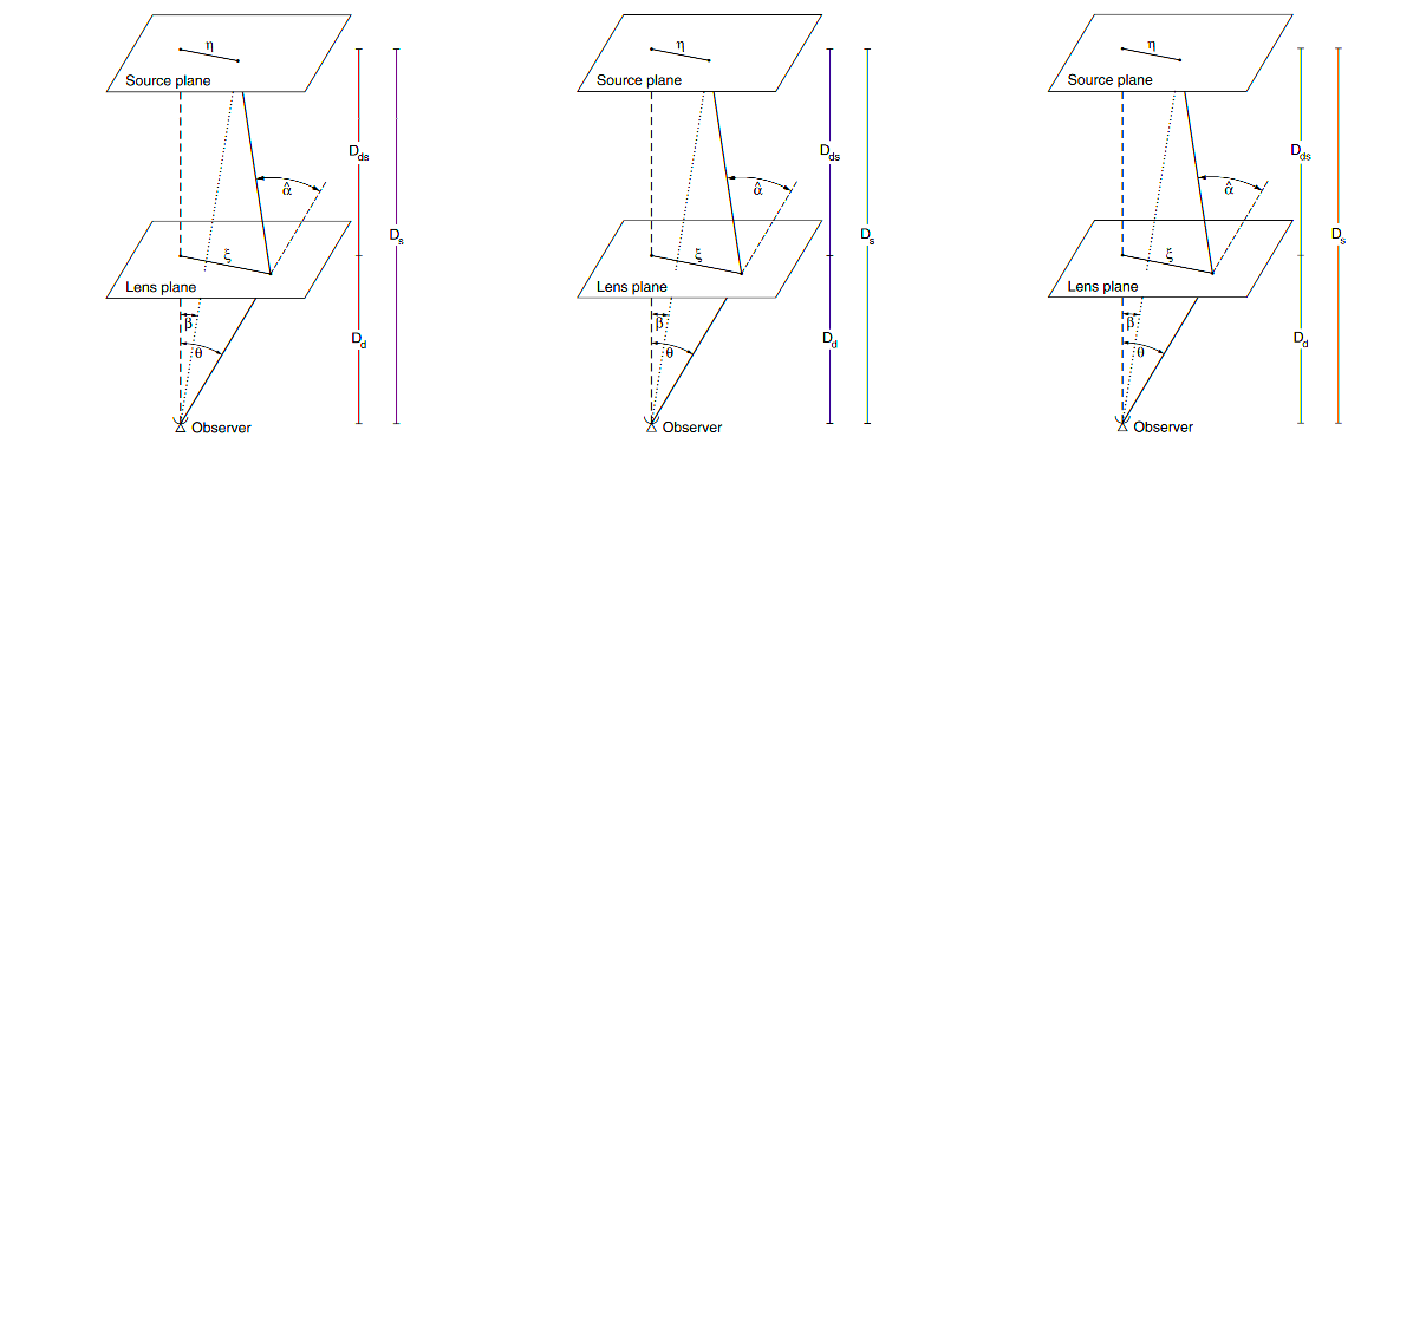
\includegraphics[width=0.5\textwidth]{grav_lensing}
      \caption[Simple sketch to gravitational lensing.] {Simple sketch to gravitational lensing ~\protect\cite{barSch_01}} %{~\protect\cite{barSch_01} } % \protect ~\cite{barSch_01}
      \label{[fig:lensing] }% \protect \cite{barSch_01}
  \end{figure} % (Bartelmann and Schneider 2001)}
  

  General Relativity predicts that when the beam of light passes through near
  the massive objects, the rays of light undergo deflection from their original path.
  This angle of deflection was predicted by Einstein's theory of General Relativity.
  According to this theory if the massive object of mass $M$ is located at a
  perpendicular distance $\xi$ (called \textbf{impact parameter}) from the line of sight
  of source and the observer then the deflection caused by that mass is given by
  \cite{sch07}
  \begin{equation}
    \hat{\alpha} = \frac{4GM}{c^2\xi}.
    \label{[eq:deflection]}
  \end{equation}

  This equation (\ref{[eq:deflection]} ) is valid only when the angle
  $\hat{\alpha} <<1  $ . In  case of gravitational lensing, the product of mass of the
  deflector and the Gravitational Constant is always the much smaller than the
  squared of velocity of light, thus making the deflection angle very small.

  For quantitative purpose,
  we can calculate the value of deflection angle for distant stars appearing near to the
  solar limb by setting the mass $M = M_{\odot}$ and radius $ R = R_{\odot}$ in the above equation to obtain the angle of deflection $\hat{\alpha} = 1.74''$. This value was tested
  in famous solar eclipse experiment in May 29, 1991 which was conceived by Sir Frank Watson Dyson, Astronomer Royal of Britain in 1917 and led by Sir Arthur Stanley Eddington
  two years later in 1919 (\cite{eclipse19}). The experiment was designed to test following hypotheses:



  \begin{itemize}

    \item{The light path is uninfluenced by gravitations.}
    \item{The law of gravitation will follow Newtonian law and will produce
            0''.87 apparent displacement}
    \item{The course of ray of light will follow Einsteins generalized
            relativity and lead to apparent displacement of 1.74''.}
  \end{itemize}
  The experiment concluded that the results were close to the Einsteins predicted
  deflection angle and thus supporting the gravitational lensing theory.

  %capranico 63 and schBar 327
  This was the deflection due to point source. We can also define the delfection
  for the extended mass with certain surface mass density $\Sigma$ as
  \begin{equation}\label{[eq:alphaHat]}
    \hat{\boldsymbol{\alpha}} (\boldsymbol{\xi} ) = \frac{4G}{c^2} \int d^2 \boldsymbol{\xi\prime}\quad  \Sigma (\boldsymbol{\xi\prime}) \quad  \frac{\boldsymbol{\xi} - \boldsymbol{\xi\prime}}{|\boldsymbol{\xi} - \boldsymbol{\xi\prime} |^2}
  \end{equation}
  Here, the \textit{surface mass density} $\boldsymbol{\Sigma}$ is defined as,
  \begin{equation}\label{[eq:surface_mass_density]}
    \boxed{
    \Sigma(\boldsymbol{\xi}) \equiv \int dr_3 \ \rho(\xi_1, \xi_2, r_3)} \quad (\text{Surface Mass Density})
  \end{equation}
  which is the mass density projected onto the lens plane, perpendicular to the
  light ray, and $r_3$ is the coordinate along the line of sight, and
  $\xi_1$, $\xi_2$ the other two perpendicular coordinates.


  %
  %
  %```````````````````````````````````````````````````````````````````````````````
  %         Subsubsection : Lens equation
  %```````````````````````````````````````````````````````````````````````````````
  %
\subsection{Lens equation}
  We consider a simplistic lensing model in which lens and the source objects are
  point objects. The observer observes the rays of light from the source at a
  distance $D_s$ which pass through the gravitational influence field of a massive
  object of mass M and distance $D_d$ located perpendicularly $\boldsymbol{\xi}$ distance away
  from line of sight (also called impact parameter).


  Let  $\boldsymbol{\eta}$  denotes the true, two-dimensional position of the
  source in the source plane and $\boldsymbol{\beta}$ is the true angular position
  of the source. This means in absence of light deflection we would have,
  \begin{equation}\label{[eq:beta]}
    \boldsymbol{\beta} = \frac{\boldsymbol{\eta} }{D_s}.
  \end{equation}
  The relation between position $\boldsymbol{\xi}$ and $\boldsymbol{\theta}$  is
  given by,
  \begin{equation}\label{[eq:theta]}
    \boldsymbol{\theta} = \frac{\boldsymbol{\xi} }{D_d}.
  \end{equation}
  This means $\boldsymbol{\theta}$ is the observed position of the source on the
  sphere relative to the position of center of the lens which is the origin of
  the coordinate system with $\boldsymbol{\xi} = 0$. Where, $D_{ds}$ is the distance of
  the source plane from the lens plane.


  Here we adopt the relation,
  \begin{equation}\label{[eq:D_ds]}
    D_{ds} = D_s - D_d.
  \end{equation}
  This relation holds true as long as the relevant distances are much smaller
  than the radius of the universe ($c/H_0$) and this is always the case for
  distances within our Galaxy and in Local Group. However, this relation no longer
  holds true for cosmological distances between source and lenses.

  From the figure (\ref{[fig:lensing]}), we can relate $\boldsymbol{\eta}$ with
  deflection angle $\boldsymbol{\alpha}$ as
  \begin{equation}\label{[eq:eta]}
    \boldsymbol{\eta} = \frac{D_s}{D_d} \boldsymbol{\xi} - D_{ds} \hat{\boldsymbol{\alpha} } (\boldsymbol{\xi} ).
  \end{equation}

  Using equation (\ref{[eq:beta]}) we can write $\boldsymbol{\beta}$ as
  \begin{equation}\label{[eq:beta2]}
    \boldsymbol{\beta} = \boldsymbol{\theta} - \frac{D_{ds}}{D_s}\  \hat{\boldsymbol{\alpha} } (D_d \boldsymbol{\theta} ).
  \end{equation}

  In this equation (\ref{[eq:beta2]}) we have some factor multiplying the
  deflection angle, so we define \textit{reduced deflection angle}
  \begin{equation}\label{[eq:alphaReduced]}
    \boxed{\boldsymbol{\alpha} (\boldsymbol{\theta} ) = \frac{D_{ds}}{D_s}\  \hat{\boldsymbol{\alpha}} (D_d \boldsymbol{\theta} )} \quad (\text{Reduced Deflection Angle})
  \end{equation}

  and then rewrite the lens equation (\ref{[eq:beta2]}) as
  \begin{equation}\label{[eq:beta3]}
     \boldsymbol{\beta} = \boldsymbol{\theta} - \boldsymbol{\alpha} (\boldsymbol{\theta} ).
  \end{equation}

  For a point mass object, using the equations (\ref{[eq:alphaHat]}) and (\ref{[eq:theta]}) the equation of reduced deflection angle (\ref{[eq:alphaReduced]})
  becomes
  \begin{equation}\label{[eq:alphaAbs]}
    \abs{\boldsymbol{\alpha} (\boldsymbol{\theta} )} = \frac{D_{ds}}{D_s}\  \frac{4GM}{c^2 D_d \abs{\boldsymbol{\theta}  }}.
  \end{equation}


%
%
%```````````````````````````````````````````````````````````````````````````````
%         Subsubsection : Convergence and Deflection Potential
%```````````````````````````````````````````````````````````````````````````````
% \texorpdfstring{$math$}{alternative} is to avoid Hyperref warning 
%                                      Token not allowed in a PDF string
\subsection{Convergence \texorpdfstring{$\kappa$ and deflection potential $\psi$}{kappaDefletionPotential}}
  % sch bar 328 Aug 22, 2017 Tue
  Then convergence is defined as the ratio of the surface mass density of the lens
  and the critical surface mass density as like

  \begin{equation}\label{[eq:kappa]}
    \boxed{\kappa (\boldsymbol{\theta} ) \equiv \frac{\Sigma (D_d \boldsymbol{\theta} )}{\Sigma_{cr}}} \quad (\text{Convergence}).
   \end{equation}
  Where, the critical surface mass density is given by
  \begin{equation}\label{[eq:crit_surf_mass_density]}
    \Sigma_{cr} = \frac{c^2}{4\pi G} \frac{D_s}{D_d D_{ds}}.
  \end{equation}
  The critical density depends on the redshift of source and lens.
  If the convergence $\kappa \geq 1$ i.e. surface density is less than critical
  surface density then we can see the multiple images of the source. If the
  value of $\kappa$ is very large it is called "strong gravitational lensing"
  and if it is only slightly greater than one, it is called "weak gravitational lensing".
  So, the value of critical mass density plays the role in distinguishing weak
  vs. strong gravitational lensing.

  Moreover, we can define scaled deflection angle in terms of convergence as
  \begin{equation}\label{[eq:alpah_kappa]}
    \boldsymbol{\alpha}(\boldsymbol{\theta} ) = \frac{1}{\pi}\ \int d^2 \theta\prime \ \kappa(\boldsymbol{\theta}\prime) \ \frac{\boldsymbol{\theta} - \boldsymbol{\theta\prime} }{\abs{\boldsymbol{\theta} - \boldsymbol{\theta\prime} }^2}\  .
  \end{equation}
  and the \textit{deflection potential} can be defined as
  \begin{equation}\label{[eq:psi]}
    \psi(\boldsymbol{\theta}) = \frac{1}{\pi}\  \int d^2 \theta\prime \ \kappa(\boldsymbol{\theta\prime} ) \ ln\abs{\boldsymbol{\theta} - \boldsymbol{\theta\prime}}.
  \end{equation}
  

%
%
%```````````````````````````````````````````````````````````````````````````````
%         Subsubsection : Multiple Images
%```````````````````````````````````````````````````````````````````````````````
%
\subsection{Multiple Images}
  We can see the multiple images of the source at different places
  $\boldsymbol{\theta}_i $ if the equation (\ref{[eq:beta3]})
  holds true for different values of the deflection angles.

  \begin{figure}[ht!]
      \centering
      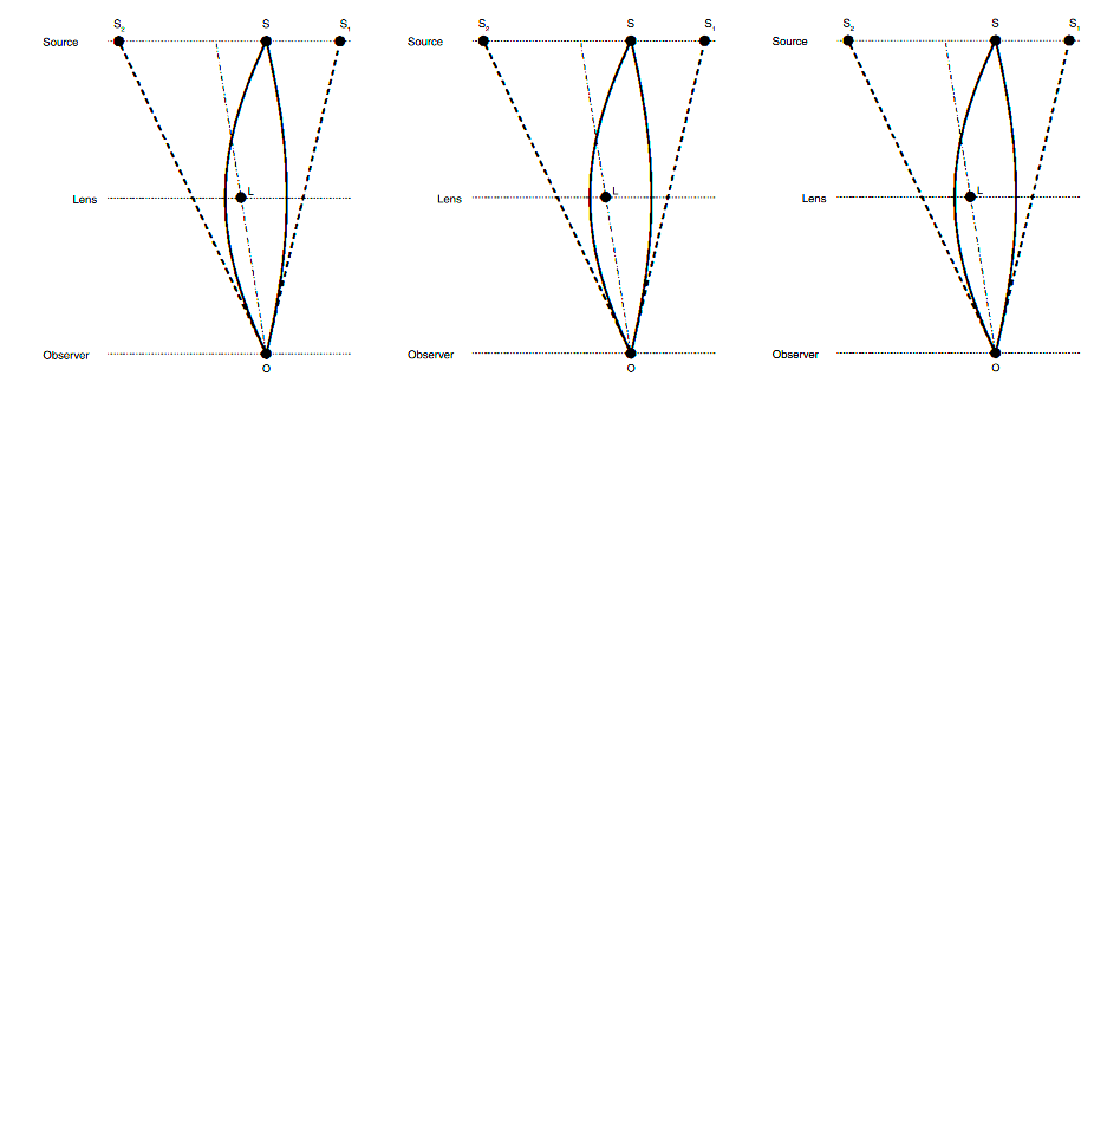
\includegraphics[width=0.5\textwidth]{multiple_images}
      \caption[Multiple images of single source]{Multiple images of single source ~\protect\cite{sch07}}
      \label{[fig:multiple_images]}
  \end{figure}

  This figure illustrates a typical situation in which there are two images $S_1$
  and $S_2$ of the single source $S$ which is lensed by the point massive object
  $L$.

  Here, if we take direction of deflection angle as pointing towards the source,
  we can write the deflection angle for the point mass (\ref{[eq:alphaAbs]}) as
  \begin{equation}\label{[eq:alpha_point_mass]}
    \boxed{\boldsymbol{\alpha} (\boldsymbol{\theta}  ) \equiv \frac{4GM}{c^2}\  \frac{D_{ds}}{D_s D_d}\  \frac{\boldsymbol{\theta} }{\abs{\boldsymbol{\theta}}^2}} \quad (\text{Reduced Deflection Angle})
  \end{equation}

  Now, we define \textit{Einstein angle} as
  \begin{equation}\label{[eq:einstein_angle]}
    \boxed{\theta_E = \sqrt{\frac{4GM}{c^2}\  \frac{D_{ds}}{D_s D_d}}} \quad (\text{Einstein Angle}).
  \end{equation}
  Then, we can rewrite the equation (\ref{[eq:alpha_point_mass]}) as
  \begin{equation}\label{[eq:beta_einstein]}
    \boldsymbol{\beta} = \boldsymbol{\theta} - {\theta_E}^2 \ \frac{\boldsymbol{\theta} }{\abs{\boldsymbol{\theta}  }^2 }
  \end{equation}

  To solve this equation (\ref{[eq:beta_einstein]}) we define two scaling factors
  \begin{equation}\label{[eq:x_y_lens]}
    y = \frac{\boldsymbol{\beta} }{\theta_E}\  ; \  x = \frac{\boldsymbol{\theta} }{\theta_E}
  \end{equation}

  Then we get
  \begin{equation}\label{[eq:y_lens]}
    \textbf{y} = \textbf{x} - \frac{\textbf{x}  }{\abs{\textbf{x}  }^2}.
  \end{equation}

  This is a quadratic equation and the solutions are given by,
  \begin{equation}\label{[eq:x_lens]}
    \textbf{x} = \frac{1}{2} (\abs{\textbf{y}} \pm \sqrt{4+ \abs{\textbf{y} }^2}) \
    \frac{\textbf{y} }{\abs{\textbf{y} }}.
  \end{equation}

  Following information can be drawn from the solution of lens equation:
  \begin{easylist}

    & {Except for the divergence condition $\theta \rightarrow 0$ any source at position $y$ has two images.}
    & {The two images are on the opposite sides of the source position when viewed from observer position.}
    & {If the source is exactly behind the lens ($\textbf{y} = 0$), we see the circular \textit{Einstein ring}. }
    & { \textit{Einstein ring} has the angular diameter $2 \theta_E $ and it gives the characteristic images separation.}
  \end{easylist}

  %
  %
  %```````````````````````````````````````````````````````````````````````````````
  %         Subsubsection : Magnification and Shear
  %```````````````````````````````````````````````````````````````````````````````
  %
\subsection{Magnification $\mu$ and shear $\gamma$ }
  The light rays in gravitational are not bent uniformly, the ones near to the
  lens are deviated more and the ones that are farther are bent in smaller
  proportion. This differential deflection gives rise to the distorted and
  magnified images of the source object.

  Let $\textbf{I}^s(\boldsymbol{\beta} )$  be the surface-brightness distribution
  of the source, then following the conservation of total surface brightness
  the observed surface-brightness distribution in the lens
  plane is given by
  \begin{equation}\label{[eq:I_theta]}
    \boldsymbol{I(\theta)} =  \textbf{I}^s \ [\boldsymbol{\beta}(\boldsymbol{\theta})].
  \end{equation}


  Now we expand the \textit{true angular position} of the source $\boldsymbol{\beta}$
  in terms of \textit{observed angular position} of the source $\boldsymbol{\theta}$
  using Taylor expansion around the central observed position $\boldsymbol{\theta_0}$
  we get

  \begin{eqnarray}\label{[eq:beta_taylor]}
    \boldsymbol{\beta}(\boldsymbol{\theta} ) = \boldsymbol{\beta}_0 + ( \boldsymbol{\theta} - \boldsymbol{\theta}_0 ) \frac{\partial\boldsymbol{\beta} }{\partial\boldsymbol{\theta}  }
  \end{eqnarray}

  Here, the term differential of $\boldsymbol{\beta}$ w.r.t. $\boldsymbol{\theta}$ is called \textit{distortion matrix}

  \begin{eqnarray}\label{[eq:dist_matrix]}
    \boxed{ \mathscr{A}(\boldsymbol{\theta} ) \equiv \frac{\partial \boldsymbol{\beta} }{ \partial \boldsymbol{\theta} }} \quad (\text{Distortion Matrix}).
  \end{eqnarray}

  Now we can write the observed surface brightness $\boldsymbol{I(\theta)}$ in terms of
  distortion matrix as
  \begin{eqnarray}\label{[eq:I_taylor]}
    \boxed{\boldsymbol{I}(\boldsymbol{\theta}) = \boldsymbol{I}^s[\beta_0 + \mathscr{A}(\boldsymbol{\theta}) (\theta - \theta_0 ) ]} \quad (\text{Observed Surface Brightness})
  \end{eqnarray}

  In terms of deflection potential $\psi$  \textit{Jacobian matrix} $\mathscr{A}$
  can be written as
  \begin{align}\label{[eq:jacobian]}
    \mathscr{A}(\boldsymbol{\theta} ) & = \frac{\partial \boldsymbol{\beta} }{ \partial \boldsymbol{\theta} } \\
      & = (\delta_{ij} - \frac{\partial^2 \psi(\boldsymbol{\theta})}{\partial \theta_i \partial \theta_j}) \nonumber \\
      & = {  \begin{pmatrix}
               1 - \psi{,11}  &-\psi_{,12}  \\
               -\psi{,21}  & 1 - \psi_{,22} \ .
            \end{pmatrix}
          }
  \end{align}

  From these deflection potential terms, we define shear components
  \begin{eqnarray}\label{[eq:shear_comps]}
    \gamma_1 &=& \frac{1}{2} (\psi_{,11} + \psi_{,22} ) \\
    \gamma_2 &=& \psi_{,12}
  \end{eqnarray}

  Here, the two components tensor $\gamma$ is called \textit{shear} and is
  given by
  \begin{eqnarray}\label{[eq:shear]}
    \boxed{\gamma \equiv \gamma_1 + i \gamma_2
           = \lvert\gamma\rvert e^{2i \phi}} \quad (\text{Shear})
  \end{eqnarray}

  Here, $\gamma_1$ and $\gamma_2$ are two components of shear as given in equation
  (\ref{[eq:shear_comps]}) and $\phi$ is the phase angle.

  The shear has two components $\gamma_1$ and $\gamma_1$ which can be expressed as
  \begin{equation}\label{[eq:shear]}
    \gamma \equiv \gamma_1 + i \gamma_2 = \lvert\gamma\rvert e^{2i \phi}.
  \end{equation}
  Also, in terms of deflection potential the shear components can be expressed as
  \begin{eqnarray}\label{[eq:shear_comp]}
    \gamma_1 &=& \frac{1}{2} (\psi_{,11} - \psi_{,22} ) \\
    \gamma_2 &=& \psi_{,12} \nonumber
  \end{eqnarray}

  Also, the convergence $\kappa$ is related to the deflection potential through
  Poisson equation
  \begin{eqnarray}\label{[eq:kappa_psi]}
    \nabla^2 \psi(\theta) = 2 \kappa(\theta).
  \end{eqnarray}

  In terms of matrix elements of deflection potential $\psi$ we can write $\kappa$ as
  \begin{eqnarray}\label{[eq:kappa_psi]}
    \boxed{\kappa = \frac{1}{2} (\psi_{,11} + \psi_{,22})} \quad (\text{Convergence})
  \end{eqnarray}

  Now we can write the distortion matrix $\mathscr{A}$ in terms of
  shear components $\gamma_1$ and $\gamma_2$ and convergence $\kappa$ as
  \begin{eqnarray}\label{[eq:A_theta]}
    \mathscr{A}(\boldsymbol{\theta}) =
    \begin{pmatrix}
      1 - \kappa - \gamma_1 & - \gamma_2  \\
      - \gamma_2 & 1 - \kappa + \gamma_1
    \end{pmatrix}
  \end{eqnarray}

  If we solve this matrix we get the eigenvalues
  \begin{eqnarray}\label{[eq:eigen]}
    eig(\mathscr{A}) = 1 - \kappa \pm \lvert g \rvert .
  \end{eqnarray}

  The equation \ref{[eq:I_taylor]} has the shape of an ellipse. This means that
  if a circular galaxy is lensed then the resulting observed image will be an
  ellipse. The semi-major and semi-minor axes of the ellipse are given by
  \begin{eqnarray}\label{[eq:semi_axes]}
    a &=& \frac{R}{1 - \kappa  - \lvert g \rvert } \\
    b &=& \frac{R}{1 - \kappa  + \lvert g \rvert }
  \end{eqnarray}

  Here, $R$ is the radius of circular source, $a$ is the semi-major axis, $b$ is semi-minor axis, and $g$ is the reduced shear
  defined as
  \begin{eqnarray}\label{[eq:g]}
    \boxed{g(\boldsymbol{\theta} ) \equiv \frac{\gamma(\boldsymbol{\theta} )}{1 - \kappa(\boldsymbol{\theta} )}} \quad (\text{Reduced Shear}).
  \end{eqnarray}

  The inverse of the determinant of the matrix $\mathscr{\alpha}$ gives the
  magnification tensor. Then we define magnification as
  \begin{eqnarray}\label{[eq:magnification]}
    \boxed{\mu(\boldsymbol{\theta}) \equiv \frac{1}{det \lvert \mathscr{A} \rvert }} \quad (\text{Magnification}).
  \end{eqnarray}